%% define the main template style for the document
\documentclass{article}

%\usepackage{nips_2017}
% to compile a camera-ready version, add the [final] option, e.g.:
\usepackage[final]{nips_2017}

\usepackage[utf8]{inputenc}
\usepackage[T1]{fontenc}
\usepackage[pagebackref=true]{hyperref}
\usepackage{url}
\usepackage{nicefrac}
\usepackage{microtype}
\usepackage[nolist,nohyperlinks]{acronym}

%% Import general packages
\usepackage{
  amsmath, amssymb, amsfonts,
  algorithmic, textcomp, listings,
  graphicx, subfig,
  booktabs, longtable
}

%% start the document, the Markdown parser takes over from this point
\begin{document}
\title{Review: A Neural Algorithm of Artistic Style}

\author{
    James C. Kauten \\
    Department of Software Engineering \\
    Auburn University \\
    Auburn, AL 36832 \\
    \texttt{jck0022@auburn.edu} \\
    \And
    Behnam Rasoolian \\
    Department of Industrial Engineering \\
    Auburn University \\
    Auburn, AL 36832 \\
    \texttt{bzr0014@auburn.edu} \\
}

\maketitle

\hypertarget{paper-summary}{%
\section{Paper Summary}\label{paper-summary}}

In their arXiv preprint, \textit{A Neural Algorithm of Artistic Style},
\cite{2015arXiv150806576G} prove a level of separability between the
\textit{content} of an image, and the \textit{style} that characterizes it.
Using a \ac{CNN} trained to classify images on the ImageNet benchmark, they
transfer the style of famous works of art, onto the content of arbitrary
photographs. To do so, they define loss functions between the activation maps
of various layers in the network that measure either content, or style loss.
Minimizing the joint loss between a noise image $\textbf{x}$ and both a
content image $\textbf{p}$ and style image $\textbf{a}$ transfers the global
features of $\textbf{p}$, with the local styles of $\textbf{a}$ onto the
noise image $\textbf{x}$. Put simply, their algorithm paints photographs using
arbitrary works of art as a palette for colors and textures.


\subsection{Content}

\subsubsection{Representation}

This work relies heavily on the understanding of convolutional layers. As a
collection of image filters, each layer extracts unique features from its
input image. As such, \cite{2015arXiv150806576G} postulate that as the layer
depth increases, the network cares more about the \textit{content} of the
image. That is to say, deeper layers have a more specific understanding of
what composes a given image, whereas the shallower layers primarily understand
the image as raw pixels. This leads to their definition of
\textit{content representation} as the activations from deep layers in the
network.

To objectively measure the difference of content between two images,
\cite{2015arXiv150806576G} define a loss function $\mathcal{L}_{content}$.
Given a content image $\textbf{p}$, a noise image $\textbf{x}$, and an
arbitrary layer $l$, the activations at $l$ for $\textbf{p}$ and $\textbf{x}$
are defined as $P^l$ and $F^l$ respectively. The squared euclidean distance
then measures the $\mathcal{L}_{content}$ loss between $P^l$ and $F^l$. Eq.
\ref{eq:content-loss} shows this loss function with an additional factor of
$\frac{1}{2}$ to simplify the formulation of the analytical gradient in Eq.
\ref{eq:content-grad}.

% TODO: note the M_l and N_l variables in the above paragraph
\begin{equation}
\label{eq:content-loss}
\mathcal{L}_{content}(\mathbf{p}, \mathbf{x}, l) =
\frac{1}{2} \sum_{i=1}^{N_l}\sum_{j=1}^{M_l}{(F^l_{ij} - P^l_{ij})^2}
\end{equation}

\begin{equation}
\label{eq:content-grad}
\frac{\partial \mathcal{L}_{content}}{\partial F^l_{ij}} =
\begin{cases}
    (F^l - P^l)_{ij} & \iff F^l_{ij} > 0 \\
    0 & \iff F^l_{ij} < 0 \\
\end{cases}
\end{equation}

\subsubsection{Reconstruction}

By back propagating the error from the $\mathcal{L}_{content}$ loss, we can
minimize the difference between a content image $\textbf{p}$ and a noise image
$\textbf{x}$ based on a given layer $l$. \cite{2015arXiv150806576G} find that
the second convolutional layer of the fourth block (\textit{block4\_conv2}) of
VGG19 produces the most desirable results. Naturally, this is assessment is
subjective to the beholders tastes.

To better understand the raw effect of this loss metric, we reconstructed a
content image by taking the content loss at five separate layers in VGG19.
We use the first convolutional layer from each of the five blocks to produce
the five content reconstructions depicted in Fig.
\ref{fig:content-reconstruction}. We can see that the first three layers
(block1\_conv1, block2\_conv1, block3\_conv1) reproduce the input image in
nearly full detail. However, the fourth and fifth layers (block4\_conv1,
block5\_conv1) reconstruct the image with looser form. Deeper layers tend to
work better for style transfer because this looser representation allows
the content to blend more smoothly with other images while still preserving
the global features.

\begin{figure}[htp]
\centering
\caption{Content Reconstruction of \textit{T\"{u}bingen, Germany}}
\label{fig:content-reconstruction}

    \begin{minipage}{0.3\linewidth}
    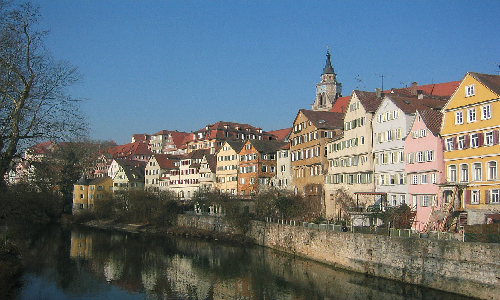
\includegraphics[width=\textwidth]{img/content/block1_conv1}
    \captionof*{figure}{block1 conv1}
    \end{minipage}
    \begin{minipage}{0.3\linewidth}
    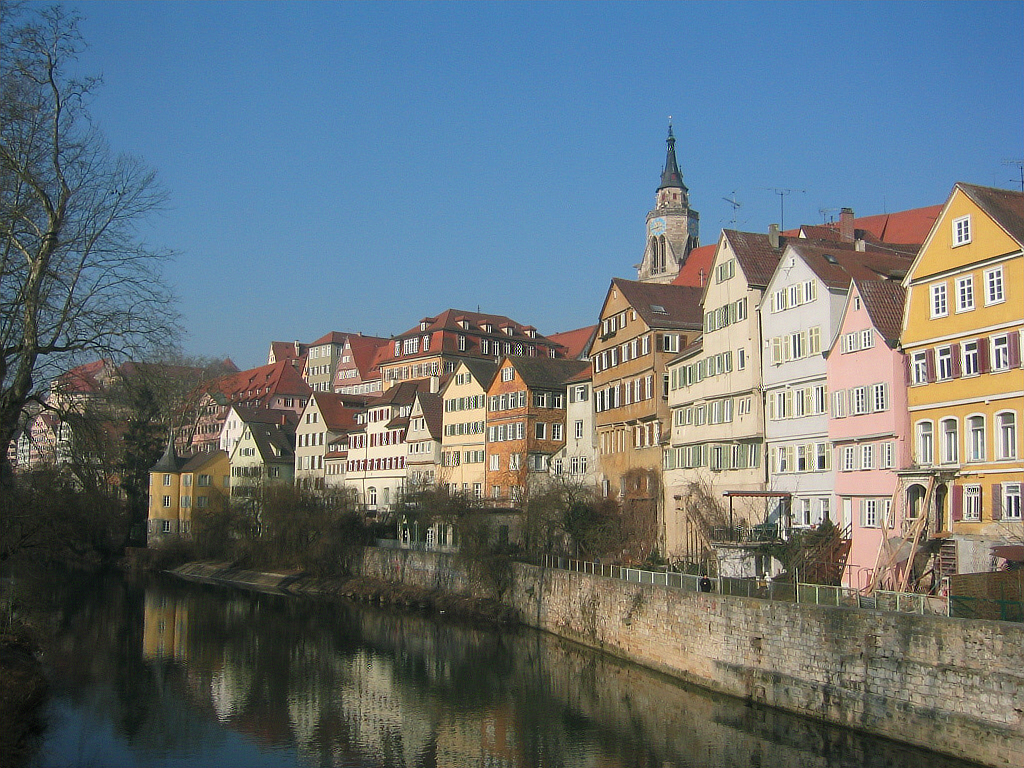
\includegraphics[width=\textwidth]{img/content/block2_conv1}
    \captionof*{figure}{block2 conv1}
    \end{minipage}
    \begin{minipage}{0.3\linewidth}
    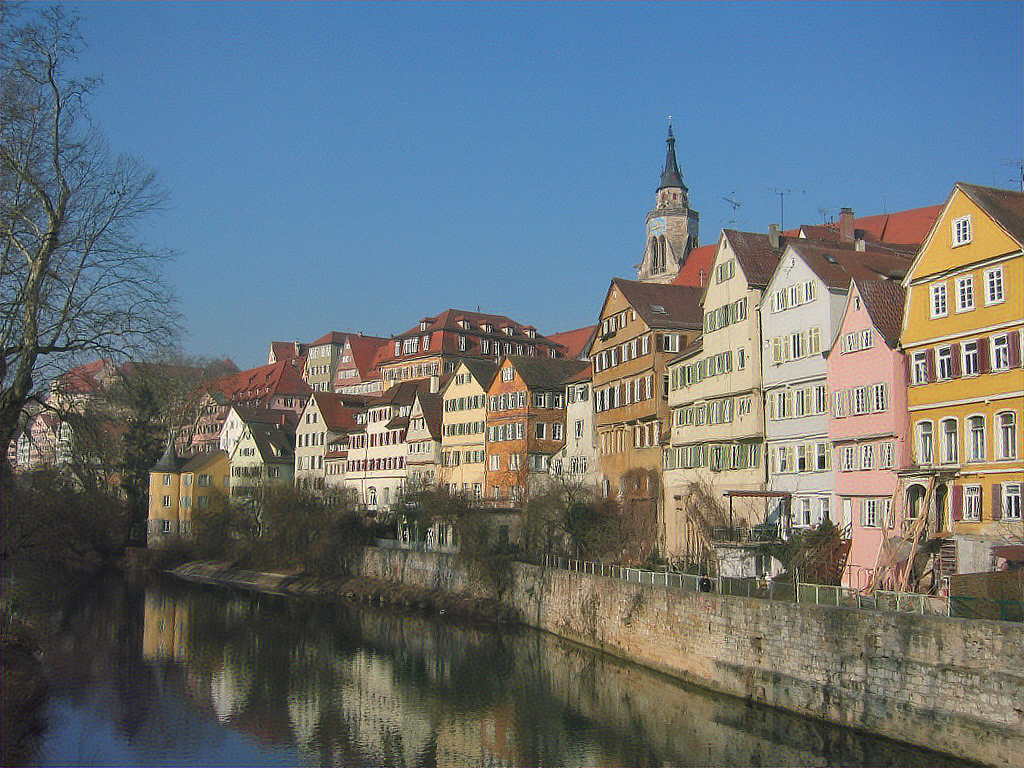
\includegraphics[width=\textwidth]{img/content/block3_conv1}
    \captionof*{figure}{block3 conv1}
    \end{minipage}

\medskip

    \begin{minipage}{0.3\linewidth}
    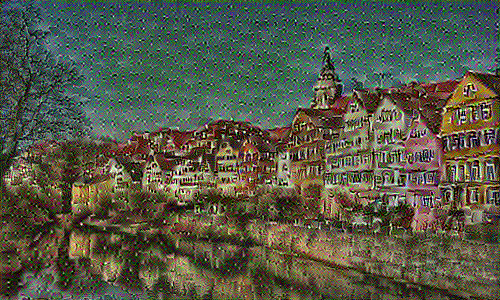
\includegraphics[width=\textwidth]{img/content/block4_conv1}
    \captionof*{figure}{block4 conv1}
    \end{minipage}
    \begin{minipage}{0.3\linewidth}
    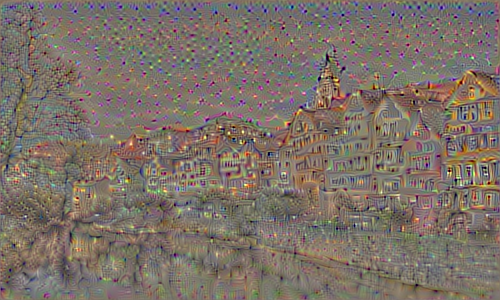
\includegraphics[width=\textwidth]{img/content/block5_conv1}
    \captionof*{figure}{block5 conv1}
    \end{minipage}

\end{figure}



\subsection{Style}

\subsubsection{Representation}

Much like the content representation, style representation relies on the
feature responses of particular layers in the \ac{CNN}. However, this
representation uses a different feature space. Converting each activation
map to a \textit{gram matrix}, allows the extraction of just the
\textit{texture} from a given image. It does so by computing the correlations
between different filters in an arbitrary convolutional layer $l$. More
simply, the gram matrix $G^l$ for an activation map $F^l$ is the inner product
of feature maps:

\begin{equation}
G_{i j}^l = \sum_{k}^{M_l} F_{i k}^l F_{j k}^l
\end{equation}

With a new feature space representation of raw texture,
\cite{2015arXiv150806576G} define an additional loss function
$\mathcal{L}_{style}$ between an artwork image $\textbf{a}$, and a noise image
$\textbf{x}$ for some convolutional layer $l$. First, the activations at $l$
for $\textbf{a}$ and $\textbf{x}$ are transformed to their respective gram
matrices $A^l$, and $G^l$. Then, much like the content loss, we define
the style loss for a given layer as the squared euclidean distance between the
gram matrices $A^l$, and $G^l$:

\begin{equation}
E_l =
\frac{1}{4 N_l^2 M_l^2}
\sum_{i=1}^{N_l}\sum_{j=1}^{M_l}
(G^l_{ij} - A^l_{ij})^2
\end{equation}

\cite{2015arXiv150806576G} incorporate multiple layers in the style loss using
a weighted sum. In their experiments, they simply use a static weight
$w_l = \frac{1}{L}$ where $L$ is the number of layers contributing to the style
loss. Eq. \ref{eq:style-loss} displays the final formulation of the
$\mathcal{L}_{style}$ loss between $\textbf{a}$ and $\textbf{x}$ for some set
of layers bounded by $L$.

\begin{equation}
\label{eq:style-loss}
\mathcal{L}_{style}(\mathbf{a}, \mathbf{x}, L) = \sum_{l=0}^L w_l E_l
\end{equation}

Finally, we derive the gradient of this loss metric in Eq.
\ref{eq:style-grad}. Again, this gradient back propagates through the network
to provide a gradient of the loss with respect to the noise image
$\textbf{x}$.

\begin{equation}
\label{eq:style-grad}
\frac{\partial E_l}{\partial F^l_{ij}} =
\begin{cases}
    \frac{1}{N^2_l M^2_l}((F^l)^T (G^l - A^l))_{ji} & \iff F^l_{ij} > 0 \\
    0 & \iff F^l_{ij} < 0 \\
\end{cases}
\end{equation}

\subsubsection{Reconstruction}

\cite{2015arXiv150806576G} use the first
convolutional layer of \textit{each} block (yielding five layers total) in
their style loss. Like the content reconstruction however, the selection of
layers for style reconstruction is subjective. To visualize the implications
of layer selection, we reconstruct style using five different sets of layers
from VGG19. Fig. \ref{fig:style-reconstruction} shows the output based on each
of the five sets. Unlike the content reconstruction, the style reconstruction
preserves none of the global content. Instead, it selects raw colors and
textures from the style, rearranging them around the new canvas $\textbf{x}$.

Like the content loss, additional layers provide a more in-depth understanding
of the style. The first convolutional layer alone seems to extract simple
points of color based on the color distribution of the style $\textbf{a}$. As
more layers contribute to the loss, the details of the texture spread and
smoothen across the noise image $\textbf{x}$.

\begin{figure}[htp]
\centering
\caption{Style Reconstruction of Vincent Van Gogh's \textit{A Starry Night}}
\label{fig:style-reconstruction}

    \begin{minipage}{0.3\linewidth}
    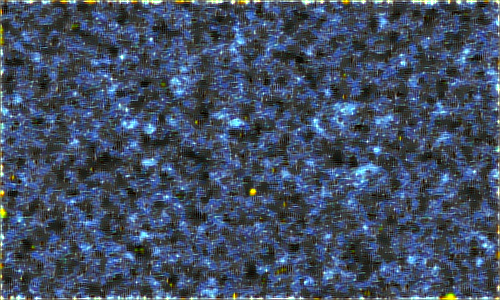
\includegraphics[width=\textwidth]{img/style/block1_conv1}
    \captionof*{figure}{block1 conv1}
    \end{minipage}
    \begin{minipage}{0.3\linewidth}
    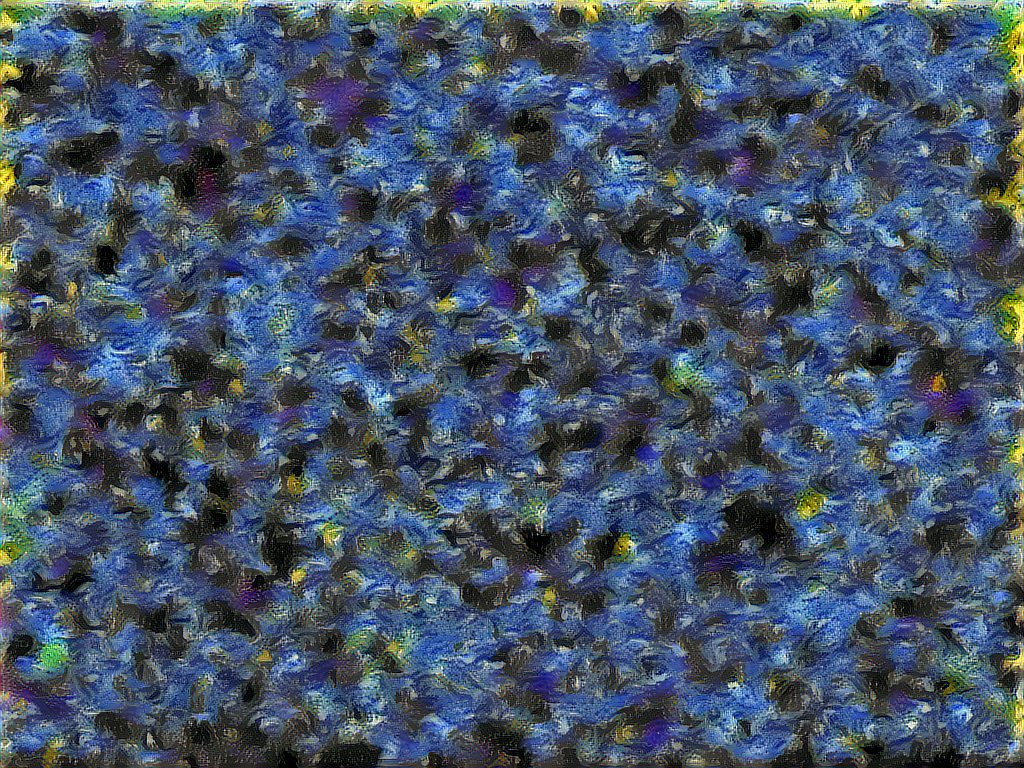
\includegraphics[width=\textwidth]{img/style/block2_conv1}
    \captionof*{figure}{block1,2 conv1}
    \end{minipage}
    \begin{minipage}{0.3\linewidth}
    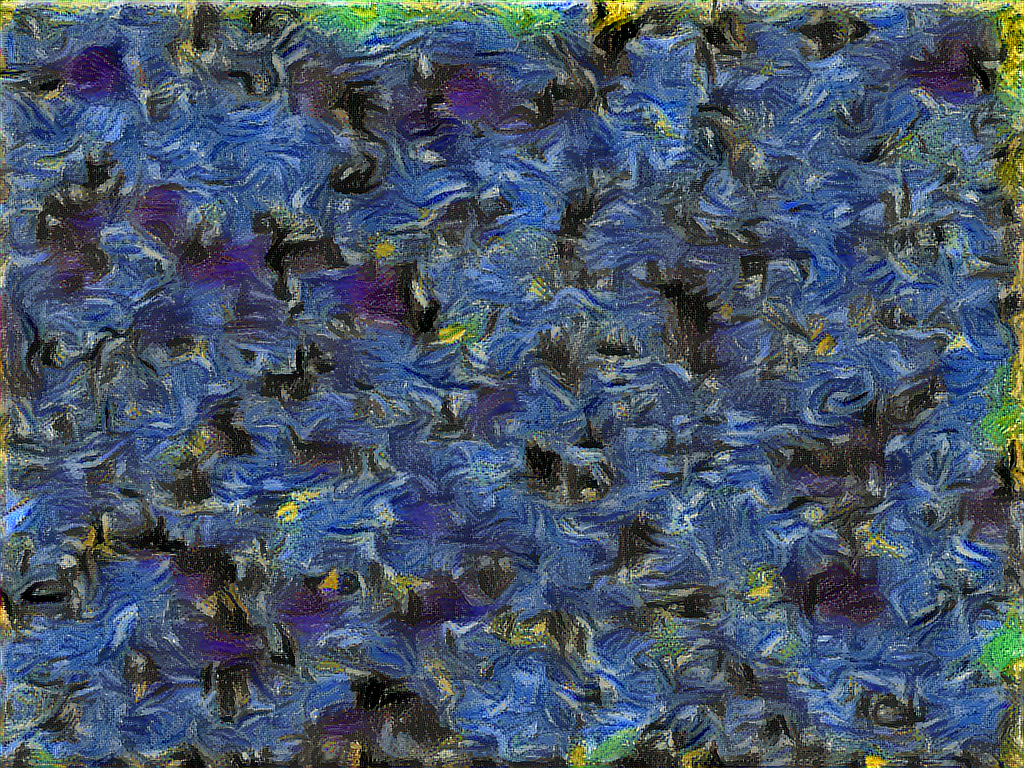
\includegraphics[width=\textwidth]{img/style/block3_conv1}
    \captionof*{figure}{block1,2,3 conv1}
    \end{minipage}

\medskip

    \begin{minipage}{0.3\linewidth}
    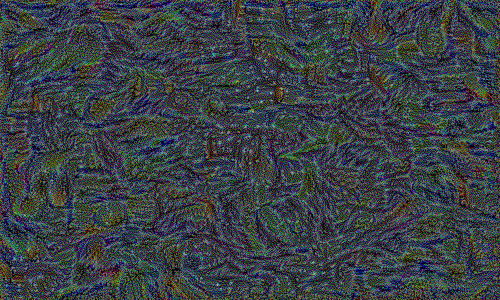
\includegraphics[width=\textwidth]{img/style/block4_conv1}
    \captionof*{figure}{block1,2,3,4 conv1}
    \end{minipage}
    \begin{minipage}{0.3\linewidth}
    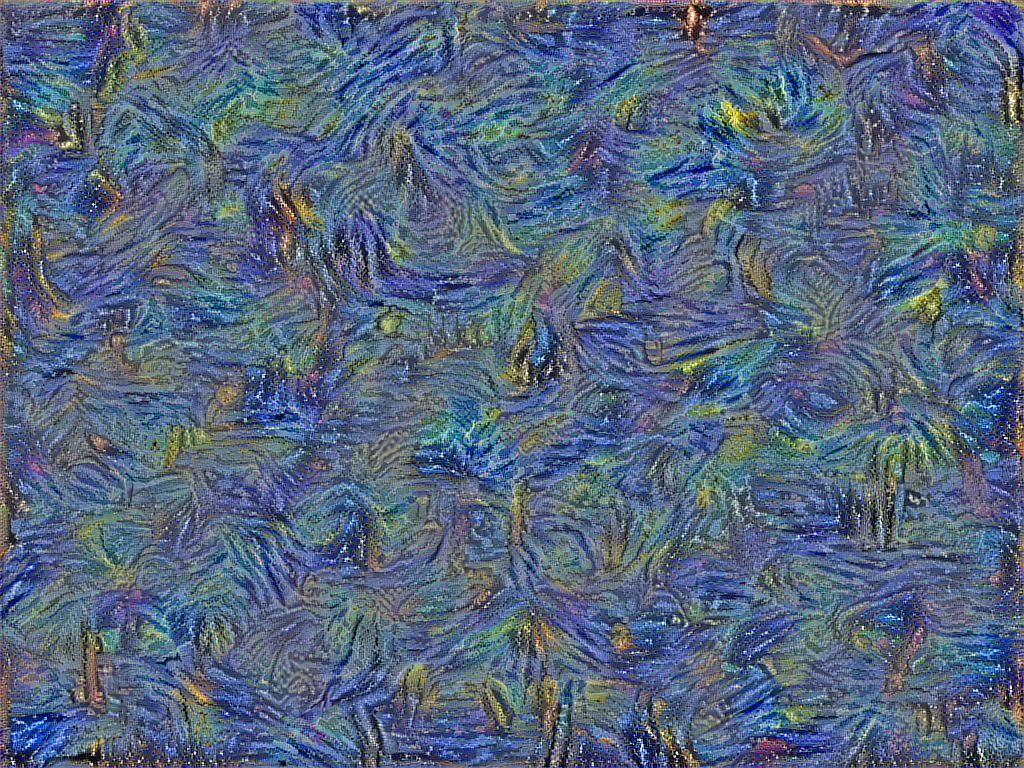
\includegraphics[width=\textwidth]{img/style/block5_conv1}
    \captionof*{figure}{block1,2,3,4,5 conv1}
    \end{minipage}

\end{figure}



\subsection{Transfer}




\hypertarget{strengths}{%
\section{Strengths}\label{strengths}}

\hypertarget{weaknesses}{%
\section{Weaknesses}\label{weaknesses}}

\hypertarget{future-work}{%
\section{Future Work}\label{future-work}}

\hypertarget{qa}{%
\section{Questions \& Answers}\label{qa}}

\bibliographystyle{my-unsrtnat}
\bibliography{references}

% a collection of Acronyms
\begin{acronym}
\acro{CNN}{Convolutional Neural Network}
\end{acronym}

\end{document}
